%%%%%%%%%%%%%%%%%%%%%%%%%%%%%%%%%%%%%%%%%
% Lachaise Assignment
% LaTeX Template
% Version 1.0 (26/6/2018)
%
% This template originates from:
% http://www.LaTeXTemplates.com
%
% Authors:
% Marion Lachaise & François Févotte
% Vel (vel@LaTeXTemplates.com)
%
% License:
% CC BY-NC-SA 3.0 (http://creativecommons.org/licenses/by-nc-sa/3.0/)
% 
%%%%%%%%%%%%%%%%%%%%%%%%%%%%%%%%%%%%%%%%%

%----------------------------------------------------------------------------------------
%	PACKAGES AND OTHER DOCUMENT CONFIGURATIONS
%----------------------------------------------------------------------------------------
\documentclass{article}


%%%%%%%%%%%%%%%%%%%%%%%%%%%%%%%%%%%%%%%%%
% Lachaise Assignment
% Structure Specification File
% Version 1.0 (26/6/2018)
%
% This template originates from:
% http://www.LaTeXTemplates.com
%
% Authors:
% Marion Lachaise & François Févotte
% Vel (vel@LaTeXTemplates.com)
%
% License:
% CC BY-NC-SA 3.0 (http://creativecommons.org/licenses/by-nc-sa/3.0/)
% 
%%%%%%%%%%%%%%%%%%%%%%%%%%%%%%%%%%%%%%%%%

%----------------------------------------------------------------------------------------
%	PACKAGES AND OTHER DOCUMENT CONFIGURATIONS
%----------------------------------------------------------------------------------------

\usepackage{amsmath,amsfonts,stmaryrd,amssymb} % Math packages
\usepackage{enumerate} % Custom item numbers for enumerations
\usepackage[ruled]{algorithm2e} % Algorithms
\usepackage[framemethod=tikz]{mdframed} % Allows defining custom boxed/framed environments
\usepackage{listings} % File listings, with syntax highlighting

\lstset{
	basicstyle=\ttfamily, % Typeset listings in monospace font
}

%----------------------------------------------------------------------------------------
%	DOCUMENT MARGINS
%----------------------------------------------------------------------------------------

\usepackage{geometry} % Required for adjusting page dimensions and margins

\geometry{
	paper=a4paper, % Paper size, change to letterpaper for US letter size
	top=2.5cm, % Top margin
	bottom=3cm, % Bottom margin
	left=2.5cm, % Left margin
	right=2.5cm, % Right margin
	headheight=14pt, % Header height
	footskip=1.5cm, % Space from the bottom margin to the baseline of the footer
	headsep=1.2cm, % Space from the top margin to the baseline of the header
	%showframe, % Uncomment to show how the type block is set on the page
}

%----------------------------------------------------------------------------------------
%	FONTS
%----------------------------------------------------------------------------------------

\usepackage{fontspec} % Required for font selection in XeLaTeX
% \usepackage{XCharter} % کامنت شد چون با فارسی سازگار نیست

%----------------------------------------------------------------------------------------
%	COMMAND LINE ENVIRONMENT
%----------------------------------------------------------------------------------------

% Usage:
% \begin{commandline}
	%	\begin{verbatim}
		%		$ ls
		%		
		%		Applications	Desktop	...
		%	\end{verbatim}
	% \end{commandline}

\mdfdefinestyle{commandline}{
	leftmargin=10pt,
	rightmargin=10pt,
	innerleftmargin=15pt,
	middlelinecolor=black!50!white,
	middlelinewidth=2pt,
	frametitlerule=false,
	backgroundcolor=black!5!white,
	frametitle={Command Line},
	frametitlefont={\normalfont\sffamily\color{white}\hspace{-1em}},
	frametitlebackgroundcolor=black!50!white,
	nobreak,
}

% Define a custom environment for command-line snapshots
\newenvironment{commandline}{
	\medskip
	\begin{mdframed}[style=commandline]
	}{
	\end{mdframed}
	\medskip
}

%----------------------------------------------------------------------------------------
%	FILE CONTENTS ENVIRONMENT
%----------------------------------------------------------------------------------------

% Usage:
% \begin{file}[optional filename, defaults to "File"]
	%	File contents, for example, with a listings environment
	% \end{file}

\mdfdefinestyle{file}{
	innertopmargin=1.6\baselineskip,
	innerbottommargin=0.8\baselineskip,
	topline=false, bottomline=false,
	leftline=false, rightline=false,
	leftmargin=2cm,
	rightmargin=2cm,
	singleextra={%
		\draw[fill=black!10!white](P)++(0,-1.2em)rectangle(P-|O);
		\node[anchor=north west]
		at(P-|O){\ttfamily\mdfilename};
		%
		\def\l{3em}
		\draw(O-|P)++(-\l,0)--++(\l,\l)--(P)--(P-|O)--(O)--cycle;
		\draw(O-|P)++(-\l,0)--++(0,\l)--++(\l,0);
	},
	nobreak,
}

% Define a custom environment for file contents
\newenvironment{file}[1][File]{ % Set the default filename to "File"
	\medskip
	\newcommand{\mdfilename}{#1}
	\begin{mdframed}[style=file]
	}{
	\end{mdframed}
	\medskip
}

%----------------------------------------------------------------------------------------
%	NUMBERED QUESTIONS ENVIRONMENT
%----------------------------------------------------------------------------------------

% Usage:
% \begin{question}[optional title]
	%	Question contents
	% \end{question}

\mdfdefinestyle{question}{
	innertopmargin=1.2\baselineskip,
	innerbottommargin=0.8\baselineskip,
	roundcorner=5pt,
	nobreak,
	singleextra={%
		\draw(P-|O)node[xshift=1em,anchor=west,fill=white,draw,rounded corners=5pt]{%
			Question \theQuestion\questionTitle};
	},
}

\newcounter{Question} % Stores the current question number that gets iterated with each new question

% Define a custom environment for numbered questions
\newenvironment{question}[1][\unskip]{
	\bigskip
	\stepcounter{Question}
	\newcommand{\questionTitle}{~#1}
	\begin{mdframed}[style=question]
	}{
	\end{mdframed}
	\medskip
}

%----------------------------------------------------------------------------------------
%	WARNING TEXT ENVIRONMENT
%----------------------------------------------------------------------------------------

% Usage:
% \begin{warn}[optional title, defaults to "Warning:"]
	%	Contents
	% \end{warn}

\mdfdefinestyle{warning}{
	topline=false, bottomline=false,
	leftline=false, rightline=false,
	nobreak,
	singleextra={%
		\draw(P-|O)++(-0.5em,0)node(tmp1){};
		\draw(P-|O)++(0.5em,0)node(tmp2){};
		\fill[black,rotate around={45:(P-|O)}](tmp1)rectangle(tmp2);
		\node at(P-|O){\color{white}\scriptsize\bf !};
		\draw[very thick](P-|O)++(0,-1em)--(O);%--(O-|P);
	}
}

% Define a custom environment for warning text
\newenvironment{warn}[1][Warning:]{ % Set the default warning to "Warning:"
	\medskip
	\begin{mdframed}[style=warning]
		\noindent{\textbf{#1}}
	}{
	\end{mdframed}
}

%----------------------------------------------------------------------------------------
%	INFORMATION ENVIRONMENT
%----------------------------------------------------------------------------------------

% Usage:
% \begin{info}[optional title, defaults to "Info:"]
	% 	contents
	% 	\end{info}

\mdfdefinestyle{info}{%
	topline=false, bottomline=false,
	leftline=false, rightline=false,
	nobreak,
	singleextra={%
		\fill[black](P-|O)circle[radius=0.4em];
		\node at(P-|O){\color{white}\scriptsize\bf i};
		\draw[very thick](P-|O)++(0,-0.8em)--(O);%--(O-|P);
	}
}

% Define a custom environment for information
\newenvironment{info}[1][Info:]{ % Set the default title to "Info:"
	\medskip
	\begin{mdframed}[style=info]
		\noindent{\textbf{#1}}
	}{
	\end{mdframed}
}

%----------------------------------------------------------------------------------------
%	PERSIAN LANGUAGE SETTINGS
%----------------------------------------------------------------------------------------

\usepackage{xepersian} % برای پشتیبانی از زبان فارسی
\settextfont{IRANSansX} % فونت فارسی (می‌توانید به Vazir یا IRANSans تغییر دهید)


\usepackage{graphicx}
\graphicspath{ {./Pics/} }
\usepackage[most]{tcolorbox}




\usepackage{listings}
\usepackage{xcolor}
% Source - https://stackoverflow.com/a/3175141
% Posted by Cloudanger, modified by community. See post 'Timeline' for change history
% Retrieved 2026-07-15, License - CC BY-SA 4.0


\usepackage{booktabs}
\usepackage{amsmath}
\usepackage{siunitx}

\usepackage{placeins}

\usepackage{pgfplots}
\pgfplotsset{compat=1.18} % تنظیم نسخه سازگاری
\usepackage{tikz} % Include the file specifying the document structure and custom commands

%----------------------------------------------------------------------------------------
%	ASSIGNMENT INFORMATION
%----------------------------------------------------------------------------------------

\title{\textbf{گزارش پروژه معماری کامپیوتر دکتر جهانگیر}} % Title of the assignment

\author{\textbf{نادر احمدی - ۴۰۳۱۰۵۶۷۴}} % Author name and email address

\date{\textbf{دانشگاه صنعتی شریف - ۱۴۰۵}} % University, school and/or department name(s) and a date

%----------------------------------------------------------------------------------------

\begin{document}

\maketitle % Print the title

%----------------------------------------------------------------------------------------
%	INTRODUCTION
%----------------------------------------------------------------------------------------
\vline


\begin{tcolorbox}[colback=blue!5!white, colframe=blue!75!black, title=توضیحات]
	برای انجام این پروژه از \textbf{پردازنده \lr{M2} }ساخت شرکت اپل استفاده شده است.
\end{tcolorbox}


\setcounter{section}{0}
\section{بخش اول: استخراج اثر انگشت ریزمعماری با زمان سنجی} % Unnumbered section
در این بخش قصد داریم موارد زیر را بررسی کنیم.
\begin{itemize}
	\item اندازه سطوح حافظه نهان \lr{(L1، L2، L3)}
	\item اندازه خط حافظه نهان \lr{(Cache Line Size)}
	\item درجه شرکت پذیری \lr{(N-way Set-Associative)}
\end{itemize}


\subsection{اندازه سطوح حافظه نهان}

در این قسمت سعی می‌کنیم با داده‌هایی با اندازه‌های $4\,\text{KB}$ تا $64\,\text{MB}$، تاخیر سطوح مختلف حافظه نهان را بسنجیم. این اندازه‌ها در هر تکرار (\lr{Iteration}) دو برابر می‌شوند تا بتوانیم مرزهای بین لایه‌های مختلف را به‌دقت تشخیص دهیم.

ابتدا آرایه‌ای از گره‌ها (\lr{Node}) ایجاد می‌شود که اندازه هر گره برابر با $128$ بایت است. تعداد گره‌ها در هر گام از تست، از تقسیم حجم کل داده بر اندازه هر گره به دست می‌آید. علت انتخاب $128$ بایت، پر کردن کامل یک خط نهان و جلوگیری از قرارگیری یک گره روی مرز دو بلوک مجزا (\lr{Misalignment}) است. البته مقدار $64$ بایت نیز مورد آزمایش قرار گرفت که به دلیل حفظ همترازی، نتایج کاملاً یکسانی حاصل شد.

اتصال بین گره‌ها بر اساس روش \lr{Pointer Chasing} پیاده‌سازی شده است به این صورت که هر گره حاوی آدرس گره بعدی بوده و زنجیره‌ای متوالی را تشکیل می‌دهند. همچنین برای غیرفعال‌سازی پیش‌بین سخت‌افزاری (\lr{Hardware Prefetcher}) و جلوگیری از کشف الگوی دسترسی توسط پردازنده، از الگوریتم \lr{Fisher-Yates Shuffle} استفاده شده است. این الگوریتم با پیمایش از انتهای آرایه به سمت ابتدا، اشاره‌گرِ گره بعدی (\lr{next}) را بین گره‌های مختلف جابه‌جا می‌کند.

\begin{figure}[h]
	\centering
	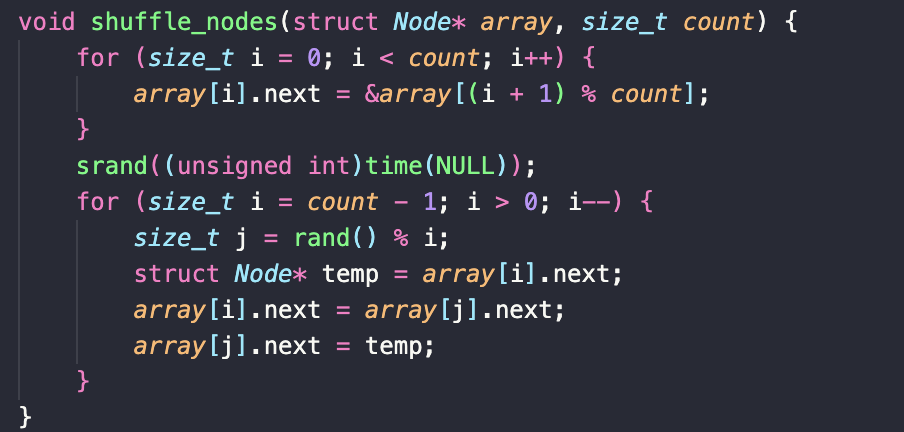
\includegraphics[width=0.5\textwidth]{1.png}
	\caption{Fisher-Yates Shuffle}
	\label{fig:}
\end{figure}

از آنجایی که حرکت در زنجیره بسیار سریع بوده و امکان اندازه گیری زمان اجرا ممکن نیست، در هر دور ۱۰ میلیون بار عمل حرکت در زنجیره را تکرار می کنیم تا زمان خروجی ملموس باشد


خروجی این مرحله به این صورت است.

\begin{figure}[h]
	\centering
	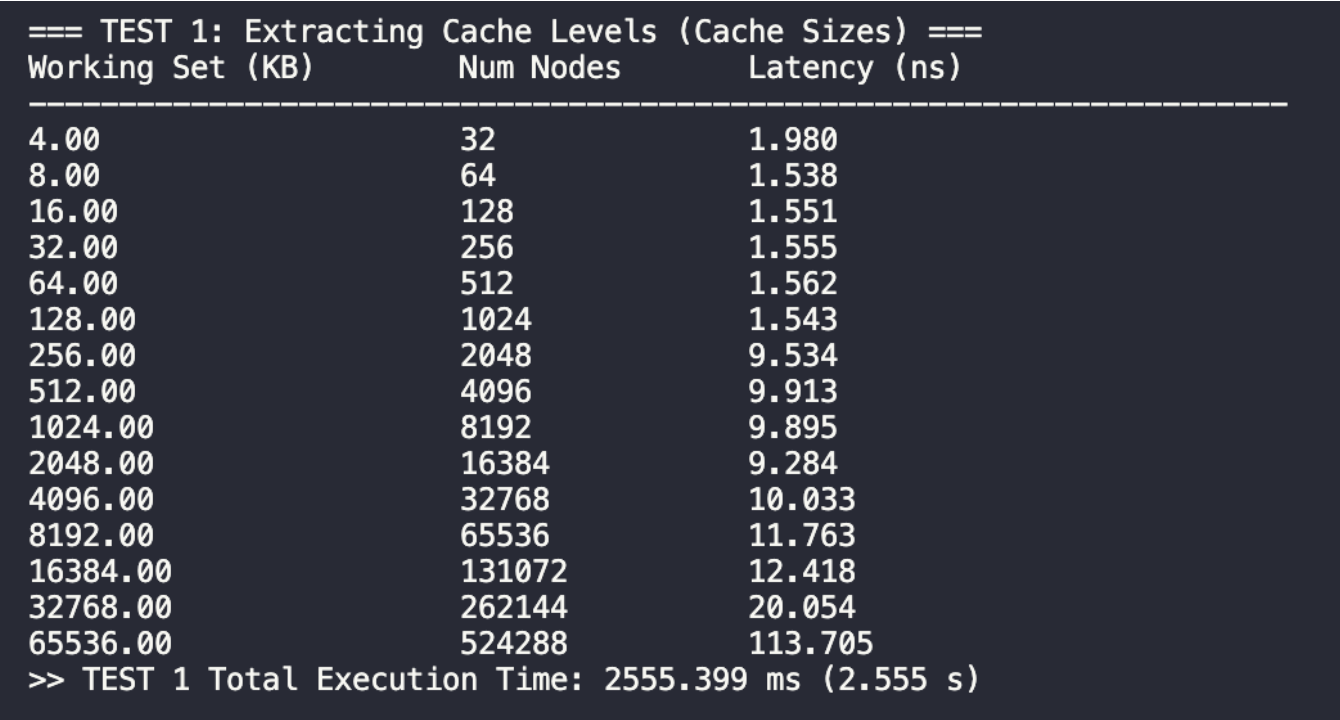
\includegraphics[width=0.6\textwidth]{T1.1_n.png}
	\caption{آزمون اندازه سطوح حافظه}
\end{figure}
\begin{latin}
\begin{figure}[htbp]
	\centering
	\begin{tikzpicture}
		\begin{axis}[
			title={Test1: Cache Layers Size},
			xlabel={Working Set - KB},
			ylabel={Latency - ns},
			% تنظیم محور افقی به صورت لگاریتمی در پایه ۲
			xmode=log,
			log basis x={2},
			xmin=4, xmax=65536,
			xtick={4, 16, 64, 128, 256, 1024, 4096, 16384, 32768, 65536},
			xticklabels={4, 16, 64, 128, 256, 1k, 4k, 16k, 32k, 64k},
			xmajorgrids=true,
			ymajorgrids=true,
			grid style=dashed,
			width=0.95\textwidth,
			height=7.5cm,
			line width=1pt,
			mark size=1.8pt,
			]
			
			% ورود داده‌های خام
			\addplot[
			color=blue,
			mark=*,
			]
			coordinates {
				(4.00, 1.980)
				(8.00, 1.538)
				(16.00, 1.551)
				(32.00, 1.555)
				(64.00, 1.562)
				(128.00, 1.543)
				(256.00, 9.534)
				(512.00, 9.913)
				(1024.00, 9.895)
				(2048.00, 9.284)
				(4096.00, 10.033)
				(8192.00, 11.763)
				(16384.00, 12.418)
				(32768.00, 20.054)
				(65536.00, 113.705)
			};
			legend{\rl{خروجی بنچمارک}}
			
			% ۱. لیبل L1 روی نقطه 128KB
			\node[anchor=south, font=\small\bfseries, color=blue!80!black] at (axis cs: 128, 3.5) {L1};
			\draw[->, >=stealth, blue!80!black] (axis cs: 128, 3.2) -- (axis cs: 128, 1.7);
			
			% ۲. لیبل L2 روی نقطه 16MB (16384KB)
			\node[anchor=south, font=\small\bfseries, color=blue!80!black] at (axis cs: 16384, 18) {L2};
			\draw[->, >=stealth, blue!80!black] (axis cs: 16384, 17.5) -- (axis cs: 16384, 13);
			
			% ۳. لیبل SLC روی نقطه 32MB (32768KB)
			\node[anchor=south, font=\small\bfseries, color=blue!80!black] at (axis cs: 32768, 32) {SLC};
			\draw[->, >=stealth, blue!80!black] (axis cs: 32768, 31) -- (axis cs: 32768, 21.5);
			
			% ۴. لیبل RAM روی آخرین نقطه (65536KB / 64MB)
			\node[anchor=east, font=\small\bfseries, color=red!80!black] at (axis cs: 65536, 113.705) {RAM \quad};
			
		\end{axis}
	\end{tikzpicture}
\end{figure}
\end{latin}

\begin{tcolorbox}[colback=green!5!white, colframe=green!75!black, title=نتایج]
	همان طور که دیده می شود تا ۱۲۸KB تاخیر واکشی داده در حدود \lr{1.5} نانوثانیه بوده است که این سطح در واقع همان \textbf{سطح اول - L1} حافظه نهان است. در ادامه از ۲۵۶KB تا ۱۶MB تاخیر در حدود \lr{9.5} الی \lr{12} نانوثانیه بوده است که این همان حافظه نهان \textbf{سطح دوم - L2 } می باشد. بعد از آن نیز جهش قابل توجهی دیده می شود که برای دسترسی به حافظه اصلی می باشد.\\
	\textbf{توجه:} سری پردازنده های M2 از حافظه نهان لایه سه بهره مند نیستند ولی دارای SLC می باشند که بین بخش های مختلف تراشه به اشتراک گذاشته شده است محدوده این حافظه نهان بین ۱۶MB تا ۳۲MB ارزیابی می شود. \\
	
	> حال باید خروجی ها را با مقادیر صحیح مقایسه کنیم. برای بدست آوردن مقادیر صحیح از دستور زیر استفاده شده است.
\begin{latin}
	\texttt{sysctl hw.perflevel0.l1dcachesize hw.perflevel0.l1icachesize hw.perflevel0.l2cachesize}
\end{latin}

خروجی این دستور به این صورت است:
\begin{latin}
	\texttt{hw.perflevel0.l1dcachesize: 131072\\
		hw.perflevel0.l1icachesize: 196608\\
		hw.perflevel0.l2cachesize: 16777216}
\end{latin}
که تا مقدار زیادی با خروجی ما یکسان است.\\ 

البته گاهی ممکن است مرز دقیق جهش تاخیر در خروجی‌های مختلف اندکی متفاوت باشد.  علت این موضوع آن است که بخشی از ظرفیت حافظه نهان سطح اول ممکن است در حین اجرا، توسط برنامه ‌های پس‌زمینهٔ سیستم‌عامل اشغال شده باشد.

\end{tcolorbox}

\subsection{اندازه خط حافظه نهان (\lr{Cache Line Size})}

در این بخش، هدف تعیین اندازه دقیق هر خط (بلوک) از حافظه نهان از طریق تغییر گام پیمایش (\lr{Stride}) است. برای انجام این تست، آرایه‌ای از داده‌ها به حجم \lr{32 MB} تخصیص داده می‌شود تا کل داده خارج از حافظه نهان L2 و درون \lr{RAM} قرار گیرد و تاخیر دسترسی به حافظه به‌وضوح قابل سنجش باشد.

در هر مرحله، حجم کل داده بر مقدار \lr{Stride} تقسیم می‌شود تا تعداد گره‌های زنجیره مشخص گردد. واضح است که با افزایش مقدار \lr{Stride}، تعداد کل گره‌های قابل پیمایش در آن چرخه کاهش می‌یابد.

\begin{figure}[h]
	\centering
	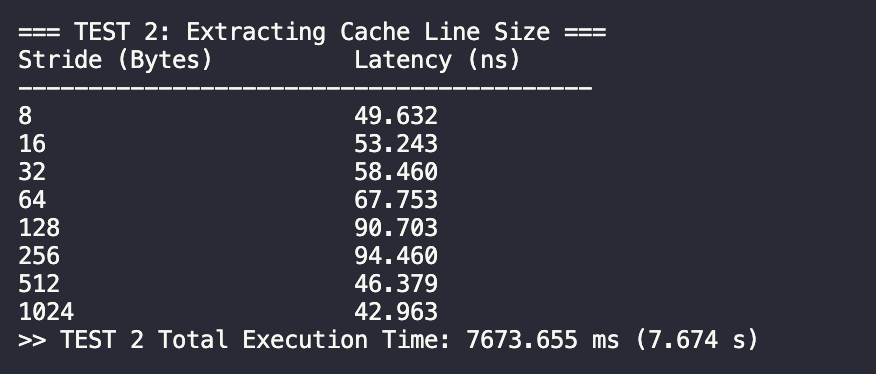
\includegraphics[width=0.6\textwidth]{T1.2_n.png}
	\caption{آزمون اندازه خطوط حافظه نهان}
	\label{fig:cache_line_size}
\end{figure}

\begin{latin}
\begin{figure}[htbp]
	\centering
	\begin{tikzpicture}
		\begin{axis}[
			title={Test2: Cache Line Size},
			xlabel={Stride - Bytes},
			ylabel={Latency - ns},
			% تنظیم محور افقی به صورت لگاریتمی پایه ۲
			xmode=log,
			log basis x={2},
			xmin=8, xmax=1024,
			xtick={8, 16, 32, 64, 128, 256, 512, 1024},
			xmajorgrids=true,
			ymajorgrids=true,
			grid style=dashed,
			width=0.95\textwidth,
			height=7.5cm,
			line width=1pt,
			mark size=1.8pt,
			]
			
			% داده‌های جدید تست ۲
			\addplot[
			color=blue!80!black,
			mark=square*,
			]
			coordinates {
				(8, 49.632)
				(16, 53.243)
				(32, 58.460)
				(64, 67.753)
				(128, 90.703)
				(256, 94.460)
				(512, 46.379)
				(1024, 42.963)
			};
			legend{\rl{خروجی بنچمارک}}
			
			
			\node[anchor=south east, font=\small\bfseries, color=blue!80!black] at (axis cs: 90, 105) {$2^7 = 128 \text{ Bytes}$ (90.70 ns)};
			\draw[->, >=stealth, line width=1pt, color=blue!80!black] (axis cs: 100, 102) -- (axis cs: 128, 90.703);
			

			
		\end{axis}
	\end{tikzpicture}
\end{figure}
\end{latin}

\begin{tcolorbox}[colback=green!5!white, colframe=green!75!black, title= نتایج]
	همان‌طور که در نمودار شکل~\ref{fig:cache_line_size} مشاهده می‌شود، در \textbf{گام ۱۲۸ بایت} یک جهش ناگهانی در تاخیر دسترسی رخ می‌دهد بنابراین می توان عدد \textbf{۱۲۸ بایت} را ‌عنوان اندازه خطوط حافظه نهان (\lr{Cache Line Size}) نتیجه‌گیری گرفت. علت کاهش تاخیر در گام‌های بعدی (\lr{Stride}های ۲۵۶ بایت به بالا) این علت است که با بزرگ‌تر شدن \lr{Stride}، تعداد کل گره‌ها به‌شدت کاهش پیدا می کند در نتیجه تعداد دسترسی ها کم می شود.
	
	جهت بررسی و صحت‌سنجی این نتیجه، دستور زیر در محیط ترمینال اجرا شد:
	
	\begin{latin}
		\texttt{sysctl hw.cachelinesize}
	\end{latin}
	
	خروجی این دستور به‌صورت زیر است:
	\begin{latin}
		\texttt{hw.cachelinesize: 128}
	\end{latin}
	که نشان می دهد نتیجه آزمایش ما درست بوده است.
\end{tcolorbox}




\subsection{درجه شرکت پذیری}

در این بخش هدف تعیین تعداد بلوک‌هایی (\lr{Ways}) است که می‌توانند به‌طور هم‌زمان درون یک مجموعه (\lr{Set}) مشخص از حافظه نهان قرار گیرند. برای این منظور، داده‌ها با فاصله ثابت $16\,\text{KB}$ از یکدیگر انتخاب می‌شوند، این کار باعث می شود که مطمئن شویم داده متعلق به یک مجموعه هستند.
سپس با افزایش گام‌به‌گام تعداد این داده‌ها از $1$ تا $16$، ظرفیت آن مجموعه مورد ارزیابی قرار می‌گیرد. تا زمانی که تعداد داده‌ها از درجه شرکت پذیری واقعی پردازنده فراتر نرفته باشد، تمامی آن‌ها درون همان مجموعه جا شده و تاخیر دسترسی در پایین‌ترین حد باقی می‌ماند. اما به محض پر شدن ظرفیت مجموعه، داده‌های جدید باعث رخ دادن خطای برخورد (\lr{Conflict Miss}) و خروج داده‌های قبلی می‌شوند که این امر با یک جهش ناگهانی در تاخیر دسترسی، درجه دقیق شرکت پذیری را مشخص می‌سازد.
خروجی این مرحله به این صورت است.

\begin{figure}[h]
	\centering
	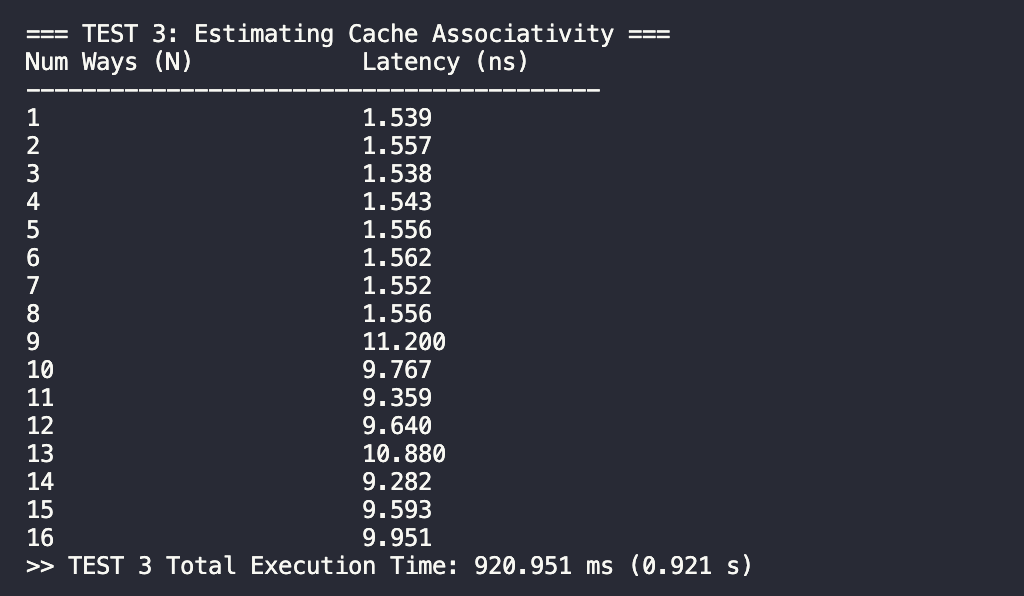
\includegraphics[width=0.6\textwidth]{T1.3_n.png}
	\caption{آزمون درجه شرکت پذیری}
\end{figure}

\begin{latin}
	
\begin{figure}[htbp]
	\centering
	\begin{tikzpicture}
		\begin{axis}[
			title={Test3: N-way Set-Associative},
			xlabel={Num Ways - N},
			ylabel={Latency - ns},
			% تنظیمات محورها
			xmin=1, xmax=16,
			ymin=0, ymax=13,
			xtick={1, 2, 3, 4, 5, 6, 7, 8, 9, 10, 11, 12, 13, 14, 15, 16},
			xmajorgrids=true,
			ymajorgrids=true,
			grid style=dashed,
			width=0.95\textwidth,
			height=7.5cm,
			line width=1pt,
			mark size=1.8pt,
			]
			
			% داده‌های جدید تست ۳
			\addplot[
			color=green!50!black,
			mark=triangle*,
			]
			coordinates {
				(1, 1.539)
				(2, 1.557)
				(3, 1.538)
				(4, 1.543)
				(5, 1.556)
				(6, 1.562)
				(7, 1.552)
				(8, 1.556)
				(9, 11.200)
				(10, 9.767)
				(11, 9.359)
				(12, 9.640)
				(13, 10.880)
				(14, 9.282)
				(15, 9.593)
				(16, 9.951)
			};
			\legend{\rl{خروجی بنچمارک}}

			\draw[->, >=stealth, line width=1pt, color=green!40!black] (axis cs: 8.8, 12.0) -- (axis cs: 9, 11.200);
			
		\end{axis}
	\end{tikzpicture}
\end{figure}
\end{latin}


\begin{tcolorbox}[colback=green!5!white, colframe=green!75!black, title=نتایج]
	همان طور که دیده می شود در درجه ۹ یک جهش ناگهانی در تاخیر داریم پس می توان نتیجه گرفت که درجه شرکت پذیری در پردازنده ما\textbf{ ۸ }می باشد. \\ با این حال خروجی دقیقی از این مقدار در اینترنت یافت نشد ولی طبق پاسخ LLM ها، درجه حافظه نهان سطح اول ۸ می باشد. پس نتیجه آزمایش درست می باشد.
	
\end{tcolorbox}

\vspace{2cm}
\section{بخش دوم: خواندن شمارنده های سخت افزاری پردازنده}


\begin{tcolorbox}[colback=blue!5!white, colframe=blue!75!black, title=توضیحات]
	از آنجایی که ابزار های پیشنهاد شده در توضیحات پروژه برای سیستم عامل مک به صورت مستقیم موجود نبود، از \textbf{ابزار Instruments موجود در Xcode} استفاده شده است. این ابزار کمک می کند که عملکرد بخش های مختلف CPU را زیر نظر گرفت.
برای رصد شمارنده های پردازنده کافیست برنامه اجرایی مورد نظر را در این ابزار انتخاب کرده و سپس با اضافه کردن Event ها به پارامتر های مورد نیاز دسترسی پیدا کرد. \\ خروجی این ابزار به فرمت \textbf{Trace} می باشد که توسط خود ابزار Instruments قابل اجراست.

\end{tcolorbox}
برای بررسی این بخش از برنامه نوشته شده در بخش اول استفاده شده است.\\
پس از اجرای برنامه، خروجی های زیر بدست آمده است که در یک جدول آورده شده است.

\begin{latin}
	\begin{table}[htbp]
		\centering
		\caption{Microarchitecture Metrics Extracted from Xcode Instruments for Process (Samples: 141,538)}
		\label{tab:microarchitecture_metrics_full}
		\begin{tabular}{llrr}
			\toprule
			\textbf{Microarchitectural Metric} & \textbf{Hardware Event} & \textbf{Total Count} & \textbf{Calculated Rate / Ratio} \\
			\midrule
			Total Executed Instructions & \texttt{INST\_ALL} & 6,443,573,748 & 100.00\% \\
			Total CPU Clock Cycles & \texttt{Cycles} & 25,523,723,774 & -- \\
			\textbf{Execution Efficiency (IPC)} & \texttt{INST\_ALL / Cycles} & -- & \textbf{0.2525} ($\text{CPI} = 3.96$) \\
			\midrule
			L1 Data Cache Miss (Load) & \texttt{L1D\_CACHE\_MISS\_LD} & 295,389,509 & -- \\
			L1 Data Cache Miss (Store) & \texttt{L1D\_CACHE\_MISS\_ST} & 23,571,344 & -- \\
			\textbf{Total L1 Data Cache Misses} & \texttt{L1D\_CACHE\_MISS (Total)} & 318,960,853 & \textbf{4.95\%} (of total instructions) \\
			\midrule
			L1 Data TLB Accesses & \texttt{L1D\_TLB\_ACCESS} & 3,533,290,451 & -- \\
			\textbf{L1 Data TLB Misses} & \texttt{L1D\_TLB\_MISS} & 163,779,190 & \textbf{4.64\%} (TLB Miss Rate) \\
			\midrule
			Branch Instructions & \texttt{INST\_BRANCH} & 1,811,420,549 & 28.11\% (of total instructions) \\
			\textbf{Branch Mispredictions} & \texttt{BRANCH\_MISPRED\_NONSPEC} & 18,873 & \textbf{0.0010\%} (Misprediction Rate) \\
			\midrule
			\textbf{Profiling Resolution} & \texttt{\# Samples} & 141,538 & \textbf{$\approx 10,011$ Hz} (Samples/sec) \\
			\bottomrule
		\end{tabular}
	\end{table}
\end{latin}


و زمان اجرای توابع مختلف این برنامه در زیر آمده است.

\begin{latin}
	\begin{table}[htbp]
		\centering
		\caption{Function Execution Time Distribution (Time Profiler Breakdown)}
		\label{tab:time_profiler_breakdown}
		\begin{tabular}{lrrr}
			\toprule
			\textbf{Benchmark Function} & \textbf{Total Time (Weight)} & \textbf{Self Time} & \textbf{\% of Total Runtime} \\
			\midrule
			\texttt{run\_cache\_line\_test} & 10.52 s & 10.34 s & \textbf{74.4\%} \\
			\texttt{run\_cache\_size\_test} & 2.67 s & 2.63 s & \textbf{18.9\%} \\
			\texttt{run\_associativity\_test} & 948.20 ms & 948.10 ms & \textbf{6.7\%} \\
			\midrule
			\textbf{Total Execution Time} & \textbf{14.14 s} & -- & \textbf{100.0\%} \\
			\bottomrule
		\end{tabular}
	\end{table}
\end{latin}

\begin{figure}[h]
	\centering
	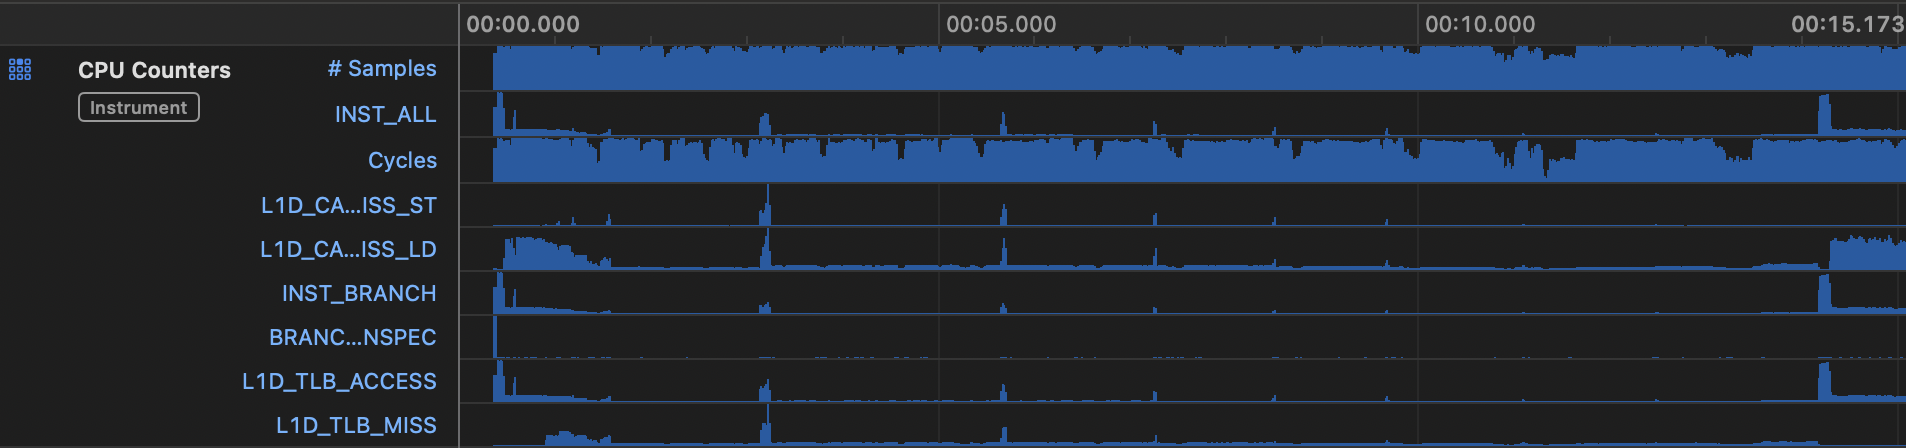
\includegraphics[width=0.75\textwidth]{Instruments_res.png}
	\caption{خط زمانی اجرای برنامه در ابزار Instruments}
\end{figure}

\subsection{پیوند با بخش اول}
حال بخش های مختلف این خط زمانی رو بررسی می کنیم.

\begin{figure}[h]
	\centering
	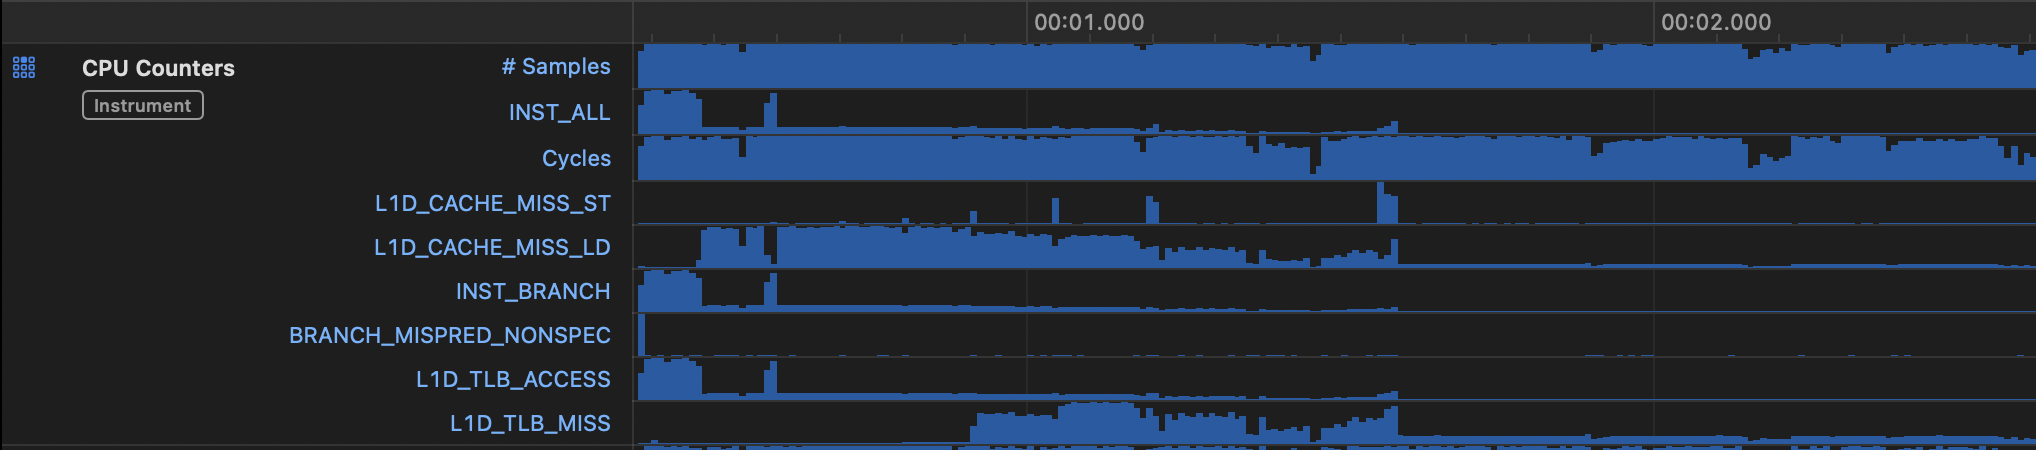
\includegraphics[width=0.75\textwidth]{T2.1.png}
	\caption{خط زمانی آزمون اندازه سطوح حافظه نهان}
\end{figure}
\FloatBarrier

همان طور که دیده می شود در ابتدا تعداد miss های لایه ۱ حافظه نهان کم است ولی بعد از بزرگ شدن حجم داده ها، ناگهان تعداد خطاها زیاد می شود که همین وضعیت در بخش اول نیز دیده شده است. علاوه بر این موضوع دیده می شود که هر چه به پایان اجرای برنامه این بخش نزدیک می شویم تراکم و ارتفاع خطاها مجدد کاهش پیدا می کند و این به این علت است که در حجم های بالا مانند \lr{16MB, 32 MB} با ایجاد هر خطا تاخیری زیادی برای بازیابی داده صرف می شود که باعث مسدود شدن پایپلاین شده و در نتیجه تراکم \lr{miss} ها کاهش پیدا کند.

\begin{figure}[h]
	\centering
	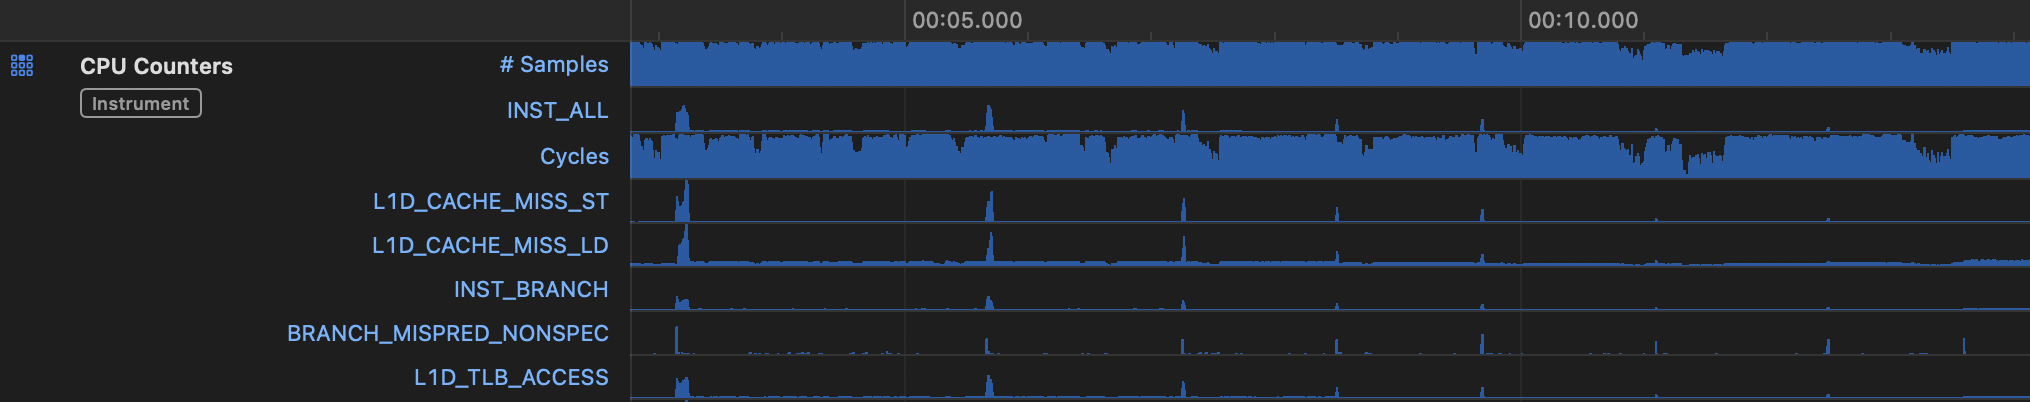
\includegraphics[width=0.75\textwidth]{T2.2.png}
	\caption{خط زمانی آزمون اندازه خط حافظه نهان}
\end{figure}
\FloatBarrier

همان‌طور که دیده می‌شود، در نقاطی از اجرا پیک‌هایی رخ داده است و در بقیه نواحی میزان خطای حافظه نهان (Miss) مقداری تقریباً یکنواخت دارد. این پیک‌ها در واقع نشان‌دهنده مراحل آماده‌سازی و درهم‌سازی (Shuffle) داده‌ها در هر دور از اجرای حلقه می‌باشند. از آنجا که در مراحل اولیه (\lr{Stride}های کوچک‌تر) تعداد گره‌ها بیشتر است، شدت و تراکم پیک‌ها نیز بیشتر دیده می‌شود. 

در بقیه نقاط نیز خطایی نسبتاً یکنواخت مشاهده می‌شود، علت آن است که به دلیل بالا بودن تاخیر بازیابی داده از \lr{RAM} (چون داده اولیه دارای \lr{32MB} است)، شدت و تعداد خطا در واحد زمان کاهش یافته و ثابت می‌ماند. نکته دیگری که دیده می‌شود، بیشتر بودن فاصله پیک‌ها در ابتدای اجرا نسبت به انتها است که علت آن، همان بار محاسباتی (Overhead) بالاتر و همچنین بیشتر بودن تعداد گره ها در چرخه های اولیه اجرا می باشد.

\begin{figure}[h]
	\centering
	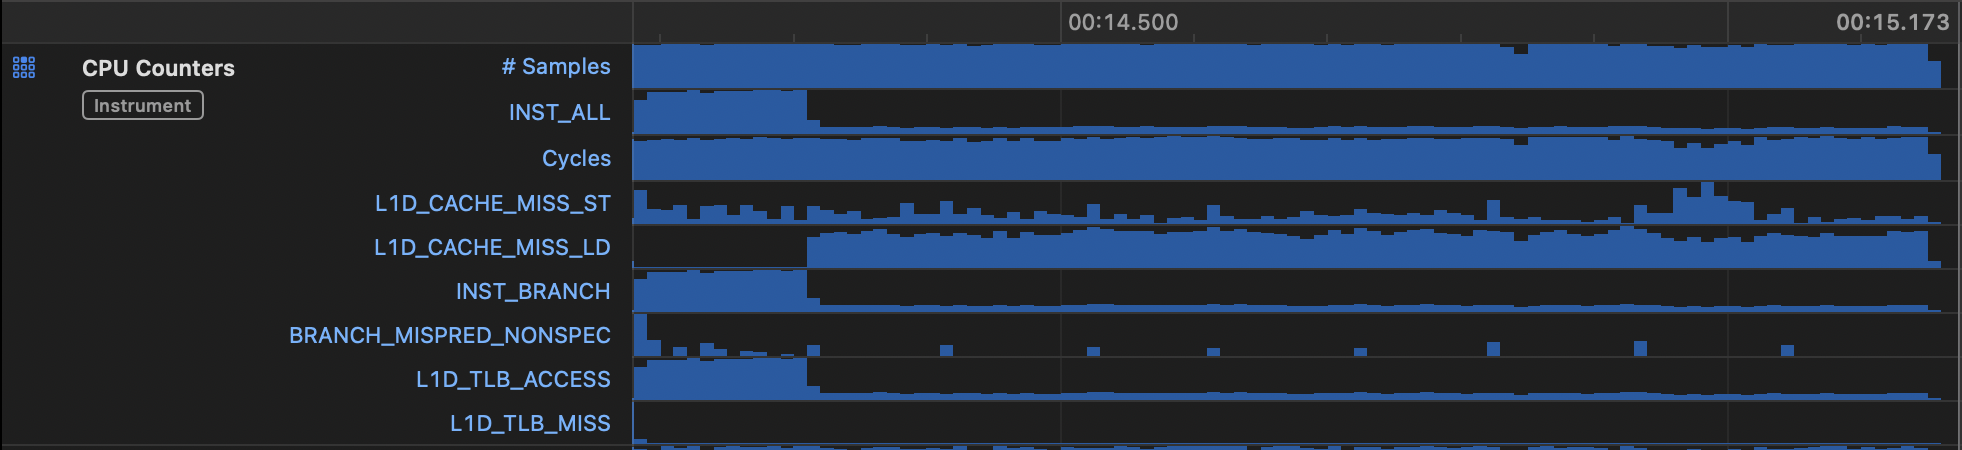
\includegraphics[width=0.75\textwidth]{T2.3.png}
	\caption{خط زمانی آزمون درجه شرکت پذیری}
\end{figure}
\FloatBarrier

در ابتدا و در درجه های کمتر به علت اینکه همه داده ها درون یک مجموعه جا می شوند، تعداد miss ها بسیار کم می باشد ولی با افزایش تعداد این درجات تمام داده ها درون یک مجموعه جا نشده و مجبور به اجرای سیاست های جایگزینی می شود و در نتیجه تعداد miss ها شدت گرفته است.



\section{بخش سوم: تحلیل و بهبود یک پدیده عملکردی}
\textbf{پدیده مورد بررسی: پیمایش سطری در برابر ستونی}


\subsection{فرضیه}
از آنجایی که داده‌های ماتریس در حافظه به صورت پشت سر هم قرار گرفتن سطرها ذخیره می‌شوند، انتظار داریم که در حالت پیمایش سطری، بنا بر اصل مجاورت مکانی، خطاها و تاخیر کمتری داشته باشیم.

\subsection{آزمایش و نتیجه‌گیری}
آزمایشی برای بررسی این پدیده طراحی شده است. در این آزمایش یک ماتریس به اندازه \lr{$4096 \times 4096$} تعریف شده که درون هر خانه داده‌ای به مقدار ۴ بایت قرار گرفته است. در حالت پیمایش سطری، محاسبه \lr{\texttt{matrix[i * SIZE + j] += i + j;}} را به صورت سطری و در پیمایش ستونی این کار را به صورت ستونی انجام می‌دهیم. \\
قطعه کدی که برای پیمایش استفاده شده در زیر آمده است:

\begin{figure}[h]
	\centering
	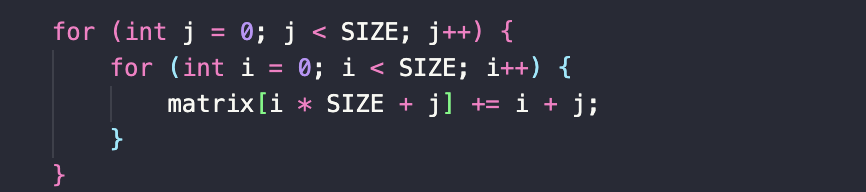
\includegraphics[width=0.75\textwidth]{T3.png}
	\caption{کد بخش پیمایش ستونی}
\end{figure}
\FloatBarrier

حال نتایج آزمایش درون \lr{CommandLine} و \lr{Instruments} در زیر آمده است:

\begin{figure}[h]
	\centering
	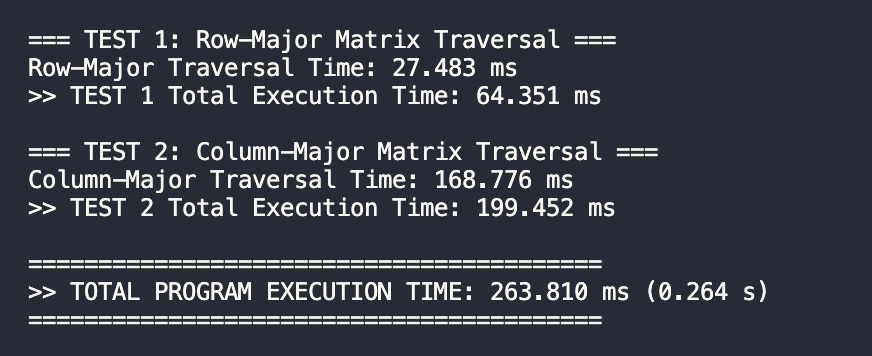
\includegraphics[width=0.75\textwidth]{T3.1.png}
	\caption{خروجی درون CommandLine}
\end{figure}
\FloatBarrier

\begin{figure}[h]
	\centering
	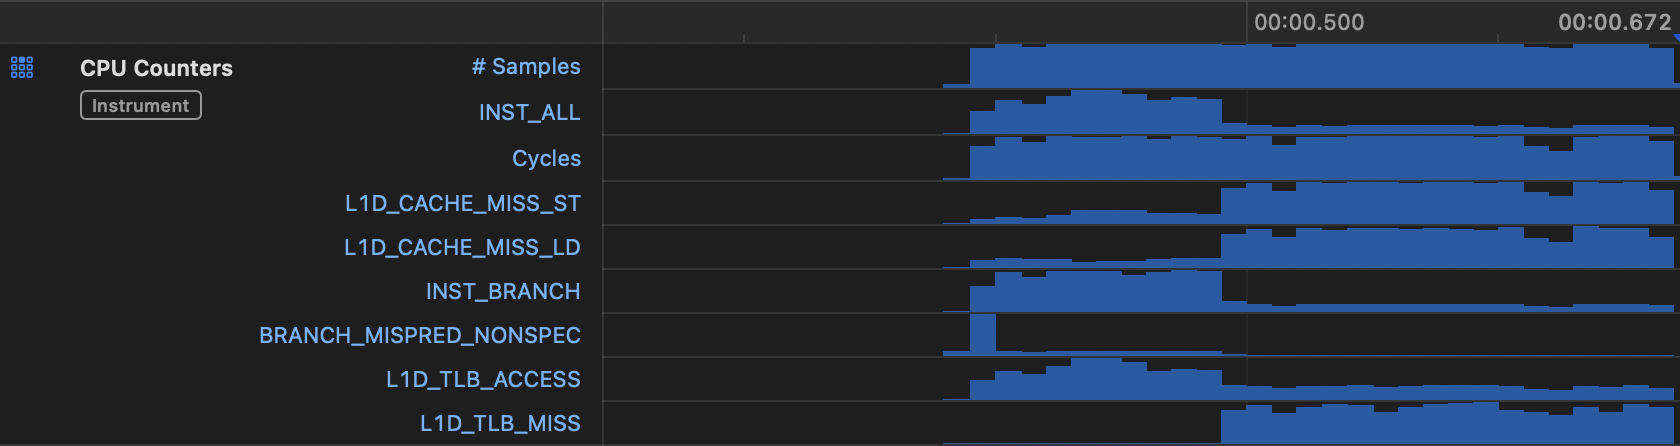
\includegraphics[width=0.75\textwidth]{T3.2.png}
	\caption{خروجی درون ابزار Instruments}
\end{figure}
\FloatBarrier

همان‌طور که دیده می‌شود، زمان اجرا و تعداد خطاهای دسترسی به حافظه نهان L1 در حالت ستونی بسیار بیشتر از حالت پیمایش سطری می‌باشد.\\
علت این مسئله به همان اصل مجاورت در حافظه نهان باز می‌گردد. هنگامی که حافظه نهان به بخشی از حافظه دسترسی پیدا می‌کند، برای افزایش نرخ موفقیت  داده‌های همسایه داده‌ی مورد رجوع را نیز درون خود ذخیره می‌کند زیرا احتمال می‌رود این داده‌ها به زودی مورد نیاز واقع شوند. حال در پیمایش سطری به علت ماهیت نحوه ذخیره‌سازی ماتریس‌ها درون حافظه، با خواندن یکی از داده‌ها، داده‌های بعدی درون آن سطر نیز وارد حافظه نهان می‌شوند و در نتیجه نرخ موفقیت  \lr{(Hit Rate)} افزایش پیدا می‌کند. از طرفی در حالت ستونی، به علت این که داده‌ها درون سطرهای مختلفی قرار دارند، خطای دسترسی \lr{(Miss Rate)} افزایش یافته و مطابق نمودار زمانی، تراکم خطاها افزایش می‌یابد.

\begin{latin}
	\begin{table}[htbp]
		\centering
		\caption{Hardware Counters - before optimzing}
		\label{tab:hardware_counters}
		\resizebox{\textwidth}{!}{%
			\begin{tabular}{llllllllll} 
				\toprule
				\textbf{Metric} & \textbf{Samples} & \textbf{INST\_ALL} & \textbf{Cycles} & \textbf{MISS\_ST} & \textbf{MISS\_LD} & \textbf{INST\_BRANCH} & \textbf{MISPRED\_NONSPEC} & \textbf{TLB\_ACCESS} & \textbf{TLB\_MISS} \\
				\midrule
				\textbf{Total} & 2747 & 1,109,406,473 & 516,911,846 & 20,379,099 & 20,228,561 & 260,724,223 & 28,546 & 690,529,492 & 128,591,428 \\
				\bottomrule
			\end{tabular}%
		}
	\end{table}
\end{latin}

\subsection{رد فرضیه‌های رقیب: خطاهای پرشی}
شاید این تصور به وجود آید که در حالت ستونی پیش‌بینی پرش‌ها دشوارتر بوده و در نتیجه تاخیر تا این حد افزایش یافته است. اما با مشاهده خروجی شمارنده‌های پردازنده متوجه می‌شویم که تعداد \lr{Branch Misprediction}ها فقط در ابتدای پیمایش سطری وجود داشته و سپس تا انتهای اجرا در یک مقدار بسیار کم ثابت می‌ماند. پس می‌توان نتیجه گرفت که این عامل تأثیر چندانی روی تاخیر به وجود آمده ندارد.


\subsection{حالت بهینه}
در این حالت برای کاهش تاخیر و خطاهای حافظه نهان در پیمایش ستونی، از روش پیمایش در پنجره‌های کوچک‌تر \lr{(Cache Tiling)} بهره گرفته‌ایم. با تعریف زیرماتریس‌های کوچک‌تر به اندازه \lr{$32 \times 32$}، پیمایش را درون این ماتریس‌های کوچک انجام می‌دهیم. در این صورت به علت کم بودن حجم این ماتریس‌ها \lr{(4 KB)}، داده‌ها به طور کامل درون حافظه نهان قرار گرفته و تاخیر کاهش پیدا می‌کند. ارقام حاصل از حالت بهینه‌یافته در زیر آمده است:


\begin{latin}
\begin{table}[htbp]
	\centering
	\caption{Hardware Counters - Optimized}
	\label{tab:hardware_counters_optimized}
	\resizebox{\textwidth}{!}{%
		\begin{tabular}{llllllllll}
			\toprule
			\textbf{Metric} & \textbf{Samples} & \textbf{INST\_ALL} & \textbf{Cycles} & \textbf{MISS\_ST} & \textbf{MISS\_LD} & \textbf{INST\_BRANCH} & \textbf{MISPRED\_NONSPEC} & \textbf{TLB\_ACCESS} & \textbf{TLB\_MISS} \\
			\midrule
			\textbf{Total} & 2208 & 1,157,513,145 & 418,807,471 & 10,803,379 & 25,678,832 & 265,005,114 & 42,767 & 661,948,878 & 4,542,589 \\
			\bottomrule
		\end{tabular}%
	}
\end{table}
\end{latin}

\FloatBarrier


حال مقایسه حالت بهینه‌یافته و حالت اولیه:

\begin{latin}
	\begin{table}[htbp]
		\centering
		\caption{Hardware Counters Comparison}
		\label{tab:hardware_counters_comparison}
		\resizebox{\textwidth}{!}{%
			\begin{tabular}{lrrr}
				\toprule
				\textbf{Hardware Metric} & \textbf{Original (Unoptimized)} & \textbf{Optimized (Tiled)} & \textbf{Improvement / Change} \\
				\midrule
				\textbf{Execution Time (ms)} & 271.60 & 217.20 & \textbf{-20.0\% (Faster)} \\
				\textbf{Samples} & 2,747 & 2,208 & -19.6\% \\
				\textbf{Total INST\_ALL} & 1,109,406,473 & 1,157,513,145 & +4.3\% (Overhead) \\
				\textbf{Total Cycles} & 516,911,846 & 418,807,471 & \textbf{-19.0\% (Faster)} \\
				\textbf{L1D\_CACHE\_MISS\_ST} & 20,379,099 & 10,803,379 & \textbf{-47.0\% (Reduced)} \\
				\textbf{L1D\_CACHE\_MISS\_LD} & 20,228,561 & 25,678,832 & +26.9\% \\
				\textbf{INST\_BRANCH} & 260,724,223 & 265,005,114 & +1.6\% \\
				\textbf{BRANCH\_MISPRED\_NONSPEC} & 28,546 & 42,767 & +14,221 ($<0.01\%$ total) \\
				\textbf{L1D\_TLB\_ACCESS} & 690,529,492 & 661,948,878 & -4.1\% \\
				\textbf{L1D\_TLB\_MISS} & 128,591,428 & 4,542,589 & \textbf{-96.5\% (Massive Drop)} \\
				\bottomrule
			\end{tabular}%
		}
	\end{table}
\end{latin}
\FloatBarrier

\subsection{پیوند میان بخش‌ها}
طبق داده‌های بخش اول متوجه شدیم که اندازه خط حافظه نهان \lr{(Cache Line)} برابر با ۱۲۸ بایت می‌باشد بنابراین با خواندن هر داده، ۱۲۸ بایت داده وارد حافظه نهان می‌شود. حال در حالت پیمایش ستونی بهینه‌نشده که اندازه هر ستون ۴۰۹۶ خانه است، پس از پیمایش کامل یک ستون، حجمی معادل \lr{$4096 \times 128 = 512\text{ KB}$} داده وارد حافظه نهان می‌شود. از آنجایی که با توجه به نتایج بخش اول، ظرفیت لایه اول حافظه نهان \lr{(L1D)} این پردازنده ۱۲۸ کیلوبایت است، پردازنده مجبور می‌شود خطوط \lr{Cache} مربوط به سطرهای اولیه را پیش از استفاده مجدد از حافظه نهان خارج کند که همین امر باعث افزایش شدید خطای دسترسی \rl{(Miss)} می‌گردد.


\end{document}
